\chapter{Graph Construction}


\section{Similarity-based methods}
\subsection{Pearson}
\label{subsec:pearson_graphs}

\subsubsection{Node and Edge Distribution}
\label{subsubsec:pearson_node_edge_distribution}

Pearson correlation was used as a linear similarity criterion for the construction of the dynamic product graphs. Unlike Spearman and Kendall, which are based on ranked or ordinal relationships, Pearson correlation measures the degree of linear co-movement between two demand series. In this setting, two products are connected when their sales deviations from their local means evolve in a similar direction and with a consistent linear pattern within the same temporal window.

This criterion is useful for identifying products whose short-term demand fluctuations are synchronized in a more direct numerical sense. Since Pearson correlation is computed after centering the observations, it is not primarily driven by the absolute sales level of each product, but by the similarity of their deviations around the local mean. Therefore, products with different average sales volumes may still be connected if their temporal movements follow a similar linear structure.

For each target product, Pearson similarities were computed over sliding windows of 15 days. In each window, the target product was compared against all active candidate products, and an edge was created whenever the Pearson similarity exceeded the selected threshold. As a result, the graph structure changes over time, allowing the neighbourhood of the target product to adapt to local variations in demand behaviour.

The temporal node and edge distribution is particularly relevant for Pearson-based graphs because linear co-movement may become stronger during specific calendar periods, such as promotional events, holidays, seasonal peaks, or other demand shocks affecting several products simultaneously. During these periods, the number of connected nodes and edges may increase, indicating that more products temporarily share similar linear demand fluctuations. In quieter periods, the graph may become sparser, suggesting that product-level demand patterns are more independent or less synchronized.
\begin{figure}
    \centering
    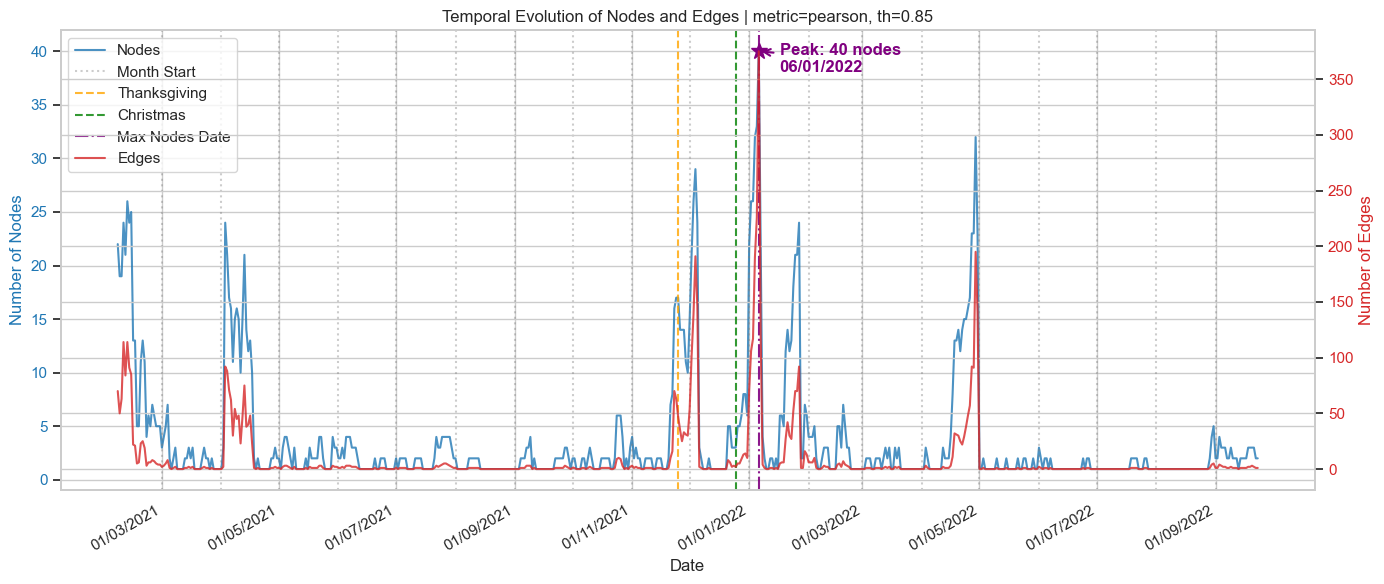
\includegraphics[width=0.5\linewidth]{figures/pearson_nodes_and_edges_distribution.png}
    \caption{Enter Caption}
    \label{fig:placeholder}
\end{figure}
Compared with rank-based measures, Pearson may be more sensitive to abrupt changes, outliers, and strong local peaks in sales. This can be advantageous when such peaks represent meaningful shared demand signals, but it can also introduce noisy edges if the similarity is driven by isolated events. Therefore, analysing the node and edge distribution across time is important to understand whether the Pearson graph captures persistent product relationships or temporary co-movements caused by short-term demand shocks.

\paragraph{Threshold Selection}

The threshold selection for Pearson was designed to evaluate different levels of graph density and selectivity. Since Pearson correlation captures linear association, lower thresholds allow the graph to include products with moderate co-movement, while higher thresholds restrict the neighbourhood to products with stronger and more synchronized demand fluctuations.

The candidate threshold grid can be expressed as:

\[
\tau \in \{\tau_{\min},\; \tau_{\min}+0.03,\; \tau_{\min}+0.06,\; \ldots,\; \tau_{\max}\}.
\]

For each threshold value, an edge is added whenever the Pearson similarity between two products is greater than or equal to $\tau$. Lower threshold values produce denser graphs and provide the forecasting model with a broader relational context. This may be useful when demand dependencies are distributed across several moderately correlated products. However, it may also increase the risk of including weak or spurious linear associations.

Higher threshold values generate sparser graphs by preserving only the strongest linear relationships. These configurations are more selective and may reduce noise in the graph structure, but they can also remove potentially useful neighbours if the threshold becomes too restrictive. This trade-off is especially relevant for Pearson correlation, since strong short-term co-movement may sometimes be caused by common calendar effects or promotional periods rather than by stable product-level relationships.

Therefore, the Pearson threshold selection procedure should be interpreted as a sensitivity analysis over alternative graph densities. By comparing forecasting performance across the threshold grid, it becomes possible to assess whether the model benefits more from dense graphs that provide wider product context or from sparse graphs that emphasize only the strongest linear co-movements.
\subsection{Spearman}
\label{subsec:spearman_graphs}

\subsubsection{Node and Edge Distribution}
\label{subsubsec:spearman_node_edge_distribution}

Spearman correlation was used as a similarity criterion to construct the dynamic product graphs. In this setting, the objective is not to connect products with similar absolute sales volumes, but rather products whose demand evolves with a similar relative ordering within each temporal window. This is particularly relevant in retail demand forecasting, since two products may operate at very different sales scales while still exhibiting comparable short-term demand movements.

For each target product, similarities were computed over sliding windows of 15 days. In each window, the target product was compared against all active candidate products, and an edge was created whenever the Spearman similarity exceeded the selected threshold. Therefore, the resulting graphs are dynamic: both the number of neighbouring nodes and the number of edges may change from one window to another, reflecting temporal variation in product relationships.

\begin{figure}
    \centering
    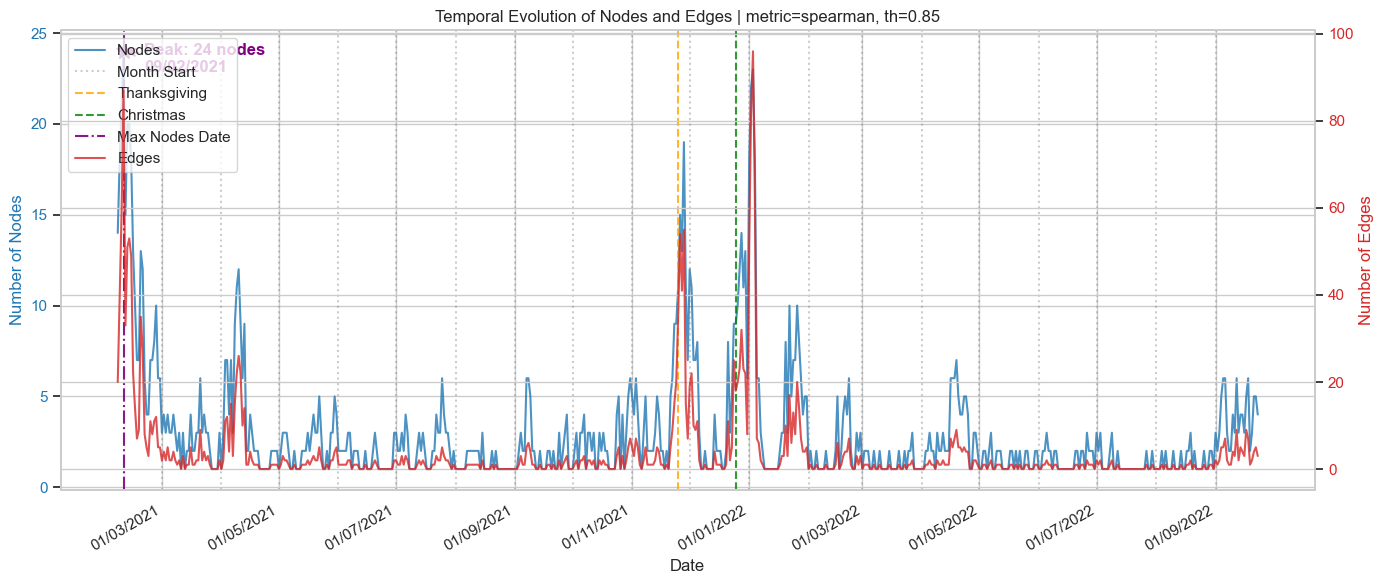
\includegraphics[width=0.5\linewidth]{node_and_edgedistribution.png}
    \caption{Spearman node and edge distribution over 15 windows
    }
    \label{fig:placeholder}
\end{figure}
Before analysing the global distribution of Spearman similarities, Figure~\ref{fig:spearman_temporal_nodes_edges} illustrates the temporal evolution of the number of nodes and edges obtained for a fixed threshold of $\tau = 0.85$. This representation is useful to understand how the selected cutoff affects graph density over time. Overall, the graph remains relatively sparse in most windows, with few neighbouring nodes connected to the target product. However, the number of nodes and edges increases sharply in specific periods, indicating temporary episodes of stronger product co-movement. These peaks are particularly visible around the beginning of the series, the Thanksgiving--Christmas period, and the transition into the following year. This behaviour suggests that product relationships are not static: they become denser during periods where demand patterns are more synchronized, likely due to seasonal effects, promotional periods, or calendar-driven consumption changes. The fact that edge peaks are more pronounced than node peaks also indicates that, when additional products enter the neighbourhood, they often form several connections among themselves, producing locally denser graph structures. Therefore, the temporal node and edge distribution confirms that even with a relatively selective threshold such as $\tau = 0.85$, the dynamic graph construction is able to capture short-term variations in relational structure rather than imposing a fixed product neighbourhood across the full time horizon.
\begin{figure}
    \centering
    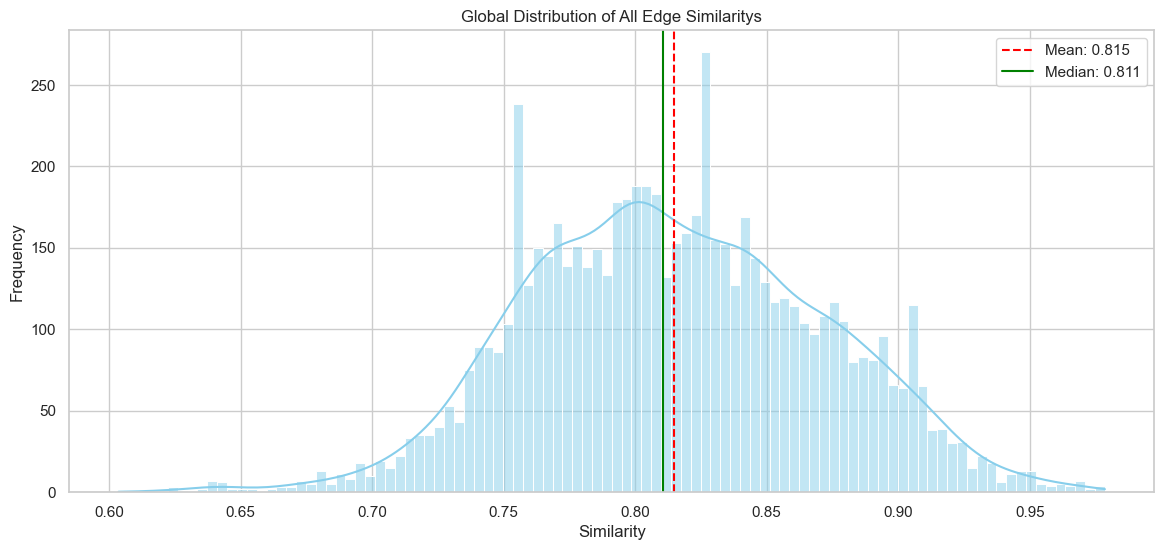
\includegraphics[width=0.5\linewidth]{figures/spearman_edge_distribution.png}
    \caption{Spearman edge similarity distribution over 15-day windows.}
    \label{fig:spearman_edge_distribution}
\end{figure}

Figure~\ref{fig:spearman_edge_distribution} presents the global distribution of Spearman edge similarities obtained across all 15-day windows. The distribution is concentrated around relatively high similarity values, with a mean of approximately 0.815 and a median of approximately 0.811. This indicates that many candidate product pairs exhibit moderate-to-strong monotonic co-movement in short temporal intervals. However, the distribution also presents a visible spread, ranging approximately from 0.60 to 0.97, which suggests that the threshold value can have a strong impact on graph density.

Lower thresholds retain a larger number of product relationships, producing denser graphs with more neighbouring nodes and more edges. While this may increase the amount of relational information available to the forecasting model, it also increases the risk of including weak or noisy associations. Conversely, higher thresholds generate sparser graphs, preserving only the strongest monotonic relationships. These graphs are more selective, but may discard potentially useful contextual information if the threshold is too restrictive.

\paragraph{Threshold Selection}

Based on the observed similarity distribution, the threshold range was defined between 0.75 and 0.91. This interval covers the central and upper regions of the distribution while avoiding extremely permissive or excessively restrictive graph configurations. Thresholds below 0.75 would include a large number of edges from the lower tail of the distribution, where similarities are weaker and more likely to represent unstable or incidental co-movements. On the other hand, thresholds above 0.91 would focus only on the extreme upper tail, generating very sparse graphs and potentially isolating the target product in several windows.

The selected interval was explored using increments of 0.03, resulting in the following threshold candidates:

\[
\tau \in \{0.75,\; 0.78,\; 0.81,\; 0.84,\; 0.87,\; 0.90\}.
\]

This grid provides a controlled way to evaluate different graph sparsity levels. The lower end of the range, around $\tau = 0.75$, favours broader neighbourhoods and allows the model to exploit a richer relational context. Intermediate values, especially around $\tau = 0.81$, are close to the empirical mean and median of the distribution, representing a balanced configuration between connectivity and selectivity. Higher values, such as $\tau = 0.87$ and $\tau = 0.90$, enforce stricter edge creation and retain only highly similar products.

Thus, the threshold selection procedure is not based on a single arbitrary cutoff, but on a sensitivity analysis over multiple graph densities. By comparing model performance across this threshold grid, it becomes possible to assess whether the forecasting model benefits more from dense relational structures, which provide broader product context, or from sparse structures, which emphasize only the strongest and most stable product relationships. This is consistent with the implemented graph construction procedure, where an edge is added when the similarity value is greater than or equal to the selected threshold. 
\subsection{Kendall}
\label{subsec:kendall_graphs}

\subsubsection{Node and Edge Distribution}
\label{subsubsec:kendall_node_edge_distribution}

Kendall correlation was also considered as a similarity criterion for the construction of the dynamic product graphs. Similarly to Spearman correlation, Kendall is based on the relative ordering of the observations rather than on their absolute magnitude. However, instead of correlating ranked values directly, Kendall evaluates the degree of concordance between pairs of observations. In this context, two products are considered similar when their demand variations preserve a consistent ordering within the same temporal window.

This makes Kendall a stricter and more conservative measure of monotonic association. While Spearman captures whether two series tend to move according to a similar ranked pattern, Kendall requires a stronger pairwise agreement between the temporal observations. As a result, Kendall-based graphs are expected to be more selective, especially when demand series contain short-term noise, local irregularities, or intermittent sales behaviour.

For each target product, Kendall similarities were computed over sliding windows of 15 days. In each window, the target product was compared with all active candidate products, and an edge was created whenever the Kendall similarity exceeded the selected threshold. Therefore, as in the Spearman case, the resulting graph sequence is dynamic: the number of neighbouring nodes and the number of edges may vary from one window to another according to the strength of the local product relationships.

\begin{figure}[h]
    \centering
    
\includegraphics[width=0.5\linewidth]{kendall_edge_distribution.png}
    \caption{Enter Caption}
    \label{fig:placeholder}
\end{figure}
The temporal evolution of nodes and edges provides an indication of how restrictive the Kendall criterion is across the demand horizon. Since Kendall is based on concordant and discordant pairs, the resulting graphs tend to retain only relationships where the relative demand ordering is highly consistent. Consequently, windows with few nodes and edges indicate periods where the target product does not share a sufficiently stable monotonic pattern with many other products. In contrast, occasional increases in graph density suggest periods of stronger synchronization between products, which may be associated with seasonal demand effects, promotional events, or broader calendar-driven consumption patterns.

\begin{figure}
    \centering
    
\includegraphics[width=0.5\linewidth]{kendall_node_and_edge_distribution.png}
    \caption{Enter Caption}
    \label{fig:placeholder}
\end{figure}

Compared with Spearman, Kendall may produce sparser graphs for equivalent threshold levels, because it penalizes local inconsistencies more strongly. This behaviour is useful from a graph construction perspective because it allows the model to focus on more robust monotonic relationships, reducing the probability of including unstable or incidental co-movements. However, excessive sparsity may also limit the amount of relational information available to the forecasting model, making threshold selection particularly important.

\paragraph{Threshold Selection}

The threshold selection for Kendall follows the same principle adopted for Spearman: different cutoff values are evaluated in order to control the trade-off between graph density and relational selectivity. Lower thresholds generate denser graphs by allowing weaker monotonic associations to be included, while higher thresholds produce sparser graphs that preserve only the most consistent product relationships.

Because Kendall correlation is generally more conservative than Spearman, the selected threshold range should be interpreted with this stricter behaviour in mind. A threshold that is moderately selective for Spearman may become highly restrictive for Kendall, since Kendall requires stronger pairwise agreement across the observations in each window. Therefore, the threshold grid is not used merely as a fixed cutoff rule, but as a sensitivity analysis over different graph sparsity levels.

The candidate thresholds can be represented as:

\[
\tau \in \{\tau_{\min},\; \tau_{\min}+0.03,\; \tau_{\min}+0.06,\; \ldots,\; \tau_{\max}\}.
\]

For each value of $\tau$, an edge is created only when the Kendall similarity is greater than or equal to the selected threshold. Lower values of $\tau$ favour broader neighbourhoods and allow the model to exploit more relational context, although with a higher risk of including weaker dependencies. Higher values of $\tau$ enforce a stricter graph structure, emphasizing only products with highly stable monotonic agreement.

Thus, the Kendall threshold selection procedure provides a controlled way to evaluate whether the forecasting model benefits from conservative relational structures. If performance improves under higher thresholds, this suggests that the model benefits from a smaller set of highly reliable neighbours. Conversely, if lower or intermediate thresholds perform better, this indicates that a broader product context may be useful even when the monotonic agreement is not as strict.
\section{Distance-based measurements}

\subsection{Data Preprocessing}

Before computing any distance-based similarity between time series, a critical preprocessing step must be addressed: the heterogeneity of sales volumes across products. In a retail setting, it is common for different stock-keeping units (SKUs) to exhibit dramatically different absolute scales — a high-volume staple product may register hundreds of units sold per day, while a niche or seasonal item may sell only a handful of units over the same period. If raw sales values are fed directly into a distance function such as the Euclidean distance, the resulting metric will be dominated by amplitude differences rather than by the underlying temporal pattern or trend structure that is relevant for graph construction.

To eliminate this scale bias, a per-item \textit{Z-score normalisation} is applied prior to computing pairwise distances. Formally, for each item $i$ with training-set time series $\mathbf{x}_i^{\text{train}} = (x_{i,1}, \ldots, x_{i,T_{\text{train}}})$, the item-specific mean $\mu_i$ and standard deviation $\sigma_i$ are estimated exclusively on the training window:

\begin{equation}
    \mu_i = \frac{1}{T_{\text{train}}} \sum_{t=1}^{T_{\text{train}}} x_{i,t}, \qquad
    \sigma_i = \sqrt{\frac{1}{T_{\text{train}}} \sum_{t=1}^{T_{\text{train}}} \left(x_{i,t} - \mu_i\right)^2}.
\end{equation}

The full time series (including validation and test periods) is then transformed as

\begin{equation}
    \tilde{x}_{i,t} = \frac{x_{i,t} - \mu_i}{\sigma_i + \varepsilon},
\end{equation}

where $\varepsilon$ is a small constant added for numerical stability. This ensures that all items are expressed in units of standard deviations from their own training mean, making the resulting series zero-centred with unit variance during the training period.

An important aspect of this procedure is that the scaler is \textit{fitted only on the training split} and then applied to the entire time axis. This discipline prevents any leakage of future statistical information into the graph construction process, which is critical given that the graphs are later used as inputs to a forecasting model. The normalised series $\tilde{\mathbf{x}}_i$ are then used in all subsequent distance computations.

\subsection{Euclidean Distance}

After normalisation, the Euclidean distance between two time series segments of length $w$ (corresponding to a sliding window) is defined as

\begin{equation}
    d_{\text{Euc}}(\mathbf{a}, \mathbf{b}) = \left\| \mathbf{a} - \mathbf{b} \right\|_2 = \sqrt{\sum_{k=1}^{w} \left(a_k - b_k\right)^2}.
\end{equation}

Because both series have been standardised to comparable scales, this quantity now reflects \textit{shape dissimilarity} rather than amplitude magnitude. Two products with similar seasonal patterns but vastly different absolute volumes will yield a small Euclidean distance after normalisation, whereas products with divergent temporal dynamics will yield a large one.


\subsection{Complexity Invariant Distance (CID)}
\label{subsec:cid_graphs}

\subsubsection{Node and Edge Distribution}
\label{subsubsec:cid_node_edge_distribution}

Complexity Invariant Distance (CID) was also considered for the construction of the dynamic product graphs. Unlike Pearson, Spearman, and Kendall, which are similarity measures, CID is a distance-based criterion. Therefore, lower values indicate stronger proximity between two product demand series, and an edge is created when the distance between two products is below a given threshold.

CID compares two time series by combining their point-wise distance with a correction factor related to their temporal complexity. In practice, this means that two products are considered close not only when their demand values are numerically close, but also when their short-term demand profiles present comparable levels of variation or roughness. This is particularly relevant in retail demand forecasting, where two products may exhibit similar global movements but differ substantially in the intensity, volatility, or irregularity of their sales patterns.

For each target product, CID distances were computed over sliding windows of 15 days. In each window, the target product was compared against all active candidate products, and an edge was created whenever the CID value was lower than or equal to the selected threshold. Therefore, as with the correlation-based approaches, the resulting graphs are dynamic: the number of neighbouring nodes and edges may change from one temporal window to another. However, because CID is distance-based, the interpretation of the threshold is reversed: higher thresholds produce denser graphs, while lower thresholds produce more selective graphs.

The node and edge distribution obtained with CID should not be interpreted as a direct equivalent of the Spearman distribution. Spearman connects products according to rank-monotonic co-movement, whereas CID connects products according to shape and complexity proximity. Consequently, CID may select different neighbours from those selected by Spearman. For example, two products may have a high Spearman correlation because their demand ranks evolve similarly, but still have a large CID distance if one series is considerably more volatile or has stronger local fluctuations. Conversely, CID may connect products with similar short-term shape and complexity even if their monotonic rank association is not among the strongest. Thus, CID provides a complementary view of product relationships, emphasizing local demand structure rather than only ordinal co-movement.

\paragraph{Threshold Selection}

Since CID is a distance metric, the threshold selection procedure was based on the condition

\[
d_{\text{CID}}(i,j) \leq \tau,
\]

where $d_{\text{CID}}(i,j)$ denotes the CID distance between products $i$ and $j$ within a given 15-day window. This is the opposite of the similarity-based metrics, where edges are created when the similarity is greater than or equal to the selected threshold.

To obtain a CID threshold grid comparable to the Spearman configuration, the cutoffs were selected by approximately matching the fraction of retained edges. Based on the filtered distributions, the following correspondence was considered:

\[
\begin{array}{c|c|c|c}
\text{Spearman threshold} & \text{Approx. retained edges} & \text{CID threshold} & \text{Approx. retained edges} \\
\hline
\rho_s \geq 0.75 & \sim 70\% & d_{\text{CID}} \leq 2.35 & \sim 70\% \\
\rho_s \geq 0.82 & \sim 35\% & d_{\text{CID}} \leq 2.15 & \sim 35\% \\
\rho_s \geq 0.85 & \sim 25\% & d_{\text{CID}} \leq 2.05 & \sim 25\% \\
\rho_s \geq 0.88 & \sim 15\% & d_{\text{CID}} \leq 1.90 & \sim 15\% \\
\rho_s \geq 0.91 & \sim 8\%  & d_{\text{CID}} \leq 1.75 & \sim 8\%
\end{array}
\]

Thus, the CID threshold candidates were defined as

\[
\tau_{\text{CID}} \in \{2.35,\; 2.15,\; 2.05,\; 1.90,\; 1.75\}.
\]

A rounded version of the same grid can also be expressed as

\[
\tau_{\text{CID}} \in \{2.40,\; 2.15,\; 2.00,\; 1.90,\; 1.75\}.
\]

This grid provides a controlled way to compare CID-based graphs with Spearman-based graphs at approximately similar density levels. The largest CID threshold, around $\tau = 2.35$ or $\tau = 2.40$, is the most permissive configuration and retains a broader product neighbourhood. This allows the forecasting model to exploit more relational information, but may also include products whose demand profiles are only moderately close in terms of shape and complexity. In contrast, the smallest threshold, $\tau = 1.75$, is the most restrictive configuration and retains only products with very close CID profiles, producing sparser graphs.

However, this matching should be interpreted carefully. The thresholds were obtained by visually comparing filtered distributions, rather than by computing exact quantiles over the complete unfiltered pool of pairwise distances and similarities. Therefore, they should be seen as approximate density-equivalent cutoffs. A stricter procedure would require recomputing both distributions without preliminary filtering and then matching the empirical percentiles directly.

More importantly, matching Spearman and CID thresholds by the retained edge fraction does not imply that both metrics select the same neighbours. It only ensures that the resulting graphs have approximately comparable densities. Spearman and CID encode different notions of product relatedness: Spearman favours products with similar rank-based monotonic evolution, while CID favours products with similar shape, amplitude proximity, and temporal complexity. Therefore, CID-based graphs may reveal alternative neighbourhoods that are not captured by rank correlation. This distinction is useful experimentally, because it allows the forecasting model to be evaluated under different assumptions about what constitutes a relevant product relationship. In the implemented graph construction procedure, this difference is reflected in the use of a distance cutoff, where candidate neighbours are selected when their CID value is lower than or equal to the global threshold. :contentReference[oaicite:0]{index=0}
\subsection{Complexity Invariant Distance (CID)}
\label{subsec:cid_graphs}

\subsubsection{Node and Edge Distribution}
\label{subsubsec:cid_node_edge_distribution}

Complexity Invariant Distance (CID) was used as a distance-based criterion for the construction of the dynamic product graphs. Unlike correlation-based measures, where larger values indicate stronger similarity, CID follows the opposite interpretation: lower values indicate that two product demand series are closer. Therefore, an edge is created when the CID distance between two products is lower than or equal to the selected threshold.

CID is particularly relevant in this context because it does not only compare the point-wise distance between two demand series, but also accounts for the complexity of their temporal evolution. As a result, two products are more likely to be connected when they present similar short-term shapes and comparable levels of variation. This means that CID may select different neighbours from correlation-based metrics such as Spearman, since it emphasizes shape-complexity proximity rather than rank-monotonic co-movement.

\begin{figure}
    \centering
    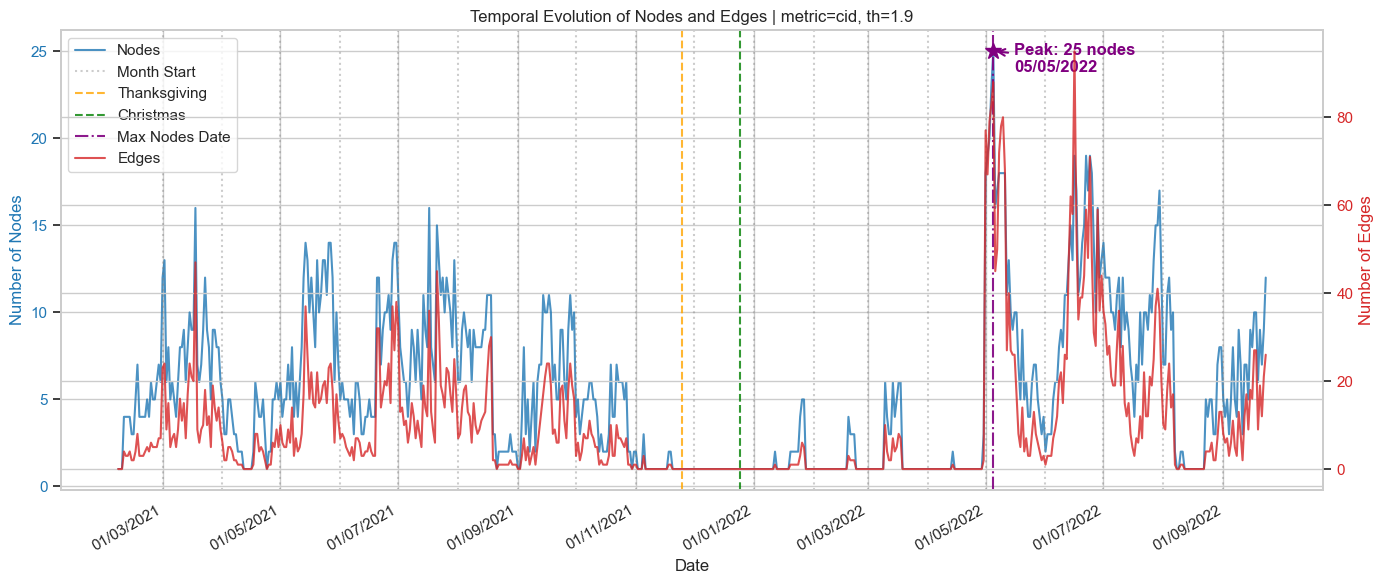
\includegraphics[width=0.75\linewidth]{figures/CID_node_and_edge_distribution.png}
    \caption{CID node and edge distribution over 15-day windows.}
    \label{fig:cid_node_edge_distribution}
\end{figure}

Figure~\ref{fig:cid_node_edge_distribution} presents the temporal evolution of the number of nodes and edges obtained with CID. This figure is useful to analyse how the graph density changes over time for a fixed distance threshold. Since CID is a distance metric, periods with more nodes and edges correspond to windows where more products exhibit similar short-term demand shapes and comparable temporal complexity. Conversely, sparse periods indicate that fewer products satisfy the distance criterion, suggesting that the target product behaves more independently or that its demand pattern differs from the remaining candidates. This temporal variability confirms that CID-based neighbourhoods are dynamic and may capture different relational structures depending on the local shape of the demand series.

\begin{figure}
    \centering
    \includegraphics[width=0.75\linewidth]{figures/cid_distance_distribution.png}
    \caption{CID distance distribution over 15-day windows.}
    \label{fig:cid_distance_distribution}
\end{figure}

Figure~\ref{fig:cid_distance_distribution} shows the global distribution of CID distances obtained across the 15-day windows. This distribution provides the basis for defining the threshold range used in the experiments. Lower CID values correspond to stronger shape-complexity proximity between products, while larger values indicate weaker relationships. Therefore, the threshold controls the sparsity of the graph in the opposite direction of correlation-based metrics: larger CID thresholds generate denser graphs, while smaller CID thresholds retain only the closest neighbours.

The threshold selection for CID was defined by approximately matching the fraction of retained edges with the Spearman threshold configuration. This allows CID-based graphs and Spearman-based graphs to be compared under similar graph-density conditions, even though the two metrics measure different types of product relationships.

Based on the filtered distributions, the following approximate correspondence was considered:

\[
\begin{array}{c|c|c|c}
\text{Spearman threshold} & \text{Approx. retained edges} & \text{CID threshold} & \text{Approx. retained edges} \\
\hline
\rho_s \geq 0.75 & \sim 70\% & d_{\text{CID}} \leq 2.35 & \sim 70\% \\
\rho_s \geq 0.82 & \sim 35\% & d_{\text{CID}} \leq 2.15 & \sim 35\% \\
\rho_s \geq 0.85 & \sim 25\% & d_{\text{CID}} \leq 2.05 & \sim 25\% \\
\rho_s \geq 0.88 & \sim 15\% & d_{\text{CID}} \leq 1.90 & \sim 15\% \\
\rho_s \geq 0.91 & \sim 8\%  & d_{\text{CID}} \leq 1.75 & \sim 8\%
\end{array}
\]

Thus, the CID threshold candidates were defined as:

\[
\tau_{\text{CID}} \in \{2.35,\; 2.15,\; 2.05,\; 1.90,\; 1.75\}.
\]

Equivalently, a rounded version of this grid can be expressed as:

\[
\tau_{\text{CID}} \in \{2.40,\; 2.15,\; 2.00,\; 1.90,\; 1.75\}.
\]

This threshold grid provides a controlled way to evaluate different CID graph densities. Higher thresholds, such as $\tau_{\text{CID}} = 2.35$ or $\tau_{\text{CID}} = 2.40$, are more permissive and retain a broader set of neighbours. Lower thresholds, such as $\tau_{\text{CID}} = 1.75$, are more restrictive and preserve only products with very close shape-complexity behaviour.

However, matching CID and Spearman thresholds by retained edge fraction does not imply that both metrics select the same neighbours. Spearman favours products with similar rank-based monotonic evolution, while CID favours products with similar shape, amplitude proximity, and temporal complexity. Therefore, CID may reveal alternative neighbourhoods that are not captured by Spearman, making it useful as a complementary graph construction criterion.


\paragraph{Threshold Selection}

\section{Elastic-based methods}
